% !TeX root = RJwrapper.tex
\title{A clustering algorithm to organize satellite hotspots data for
the purpose of tracking bushfires remotely}
\author{by Weihao Li, Emily Dodwell, and Dianne Cook}

\maketitle

\abstract{%
An abstract of less than 150 words.
}

\hypertarget{introduction}{%
\subsection{Introduction}\label{introduction}}

The 2019-2020 Australia bushfire season was catastrophic in the scale of
damage caused to agricultural resources, property, infrastructure, and
ecological systems. By the end of 2020, the devastation attributable to
these Black Summer fires included 33 lives lost, almost 19 million
hectares of land burned, over 3,000 homes destroyed and AUD \$1.7
billion in insurance losses, as well as an estimated 1 billion animals
killed, including half of Kangaroo Island's population of koalas
\citep{Filkov2020}. According to \citet{climate2020}, 2019 was the
warmest year on record in Australia and capped off a period from
2013-2019 that represents seven of the nine warmest years. There is
concern and expectation that impacts of climate change -- including more
extreme temperatures, persistent drought, and changes in plant growth
and landscape drying -- will worsen conditions for extreme bushfires
\citep[\citet{Deb2020}]{climate2020}. Contributing to the problem is
that dry lightning represents the main source of natural ignition, and
fires that start in remote areas deep in the temperate forests are
difficult to access and monitor \citep{Abram2021}. Therefore,
opportunities to detect fire ignitions, monitor bushfire spread, and
understand movement patterns in remote areas are important for
developing effective strategies to mitigate bushfire impact.

Remote satellite data provides a potential solution to the challenge of
active fire detection and monitoring, and the Himawari-8 satellite
represents a significant improvement in the technology by which this can
be done. Launched in 2015 by the Japan Meteorological Agency, its
10-minute temporal resolution enables almost real-time monitoring of
fires across East Asia and Australia. For this reason, development of
algorithms to process pixels of its satellite imagery into hotspots --
i.e.~pixels that represent likely fires -- is an active area of research
(see for example \citet{Xu2017}, \citet{Wickramasinghe2016},
\citet{Jang2019}). We make use of the Japan Aerospace Exploration Agency
(JAXA) wildfire product \citep{jaxa} that identifies the location and
fire radiative power (FRP) of hotspots according to an algorithm
developed by \citet{Kurihara2020}.

Detection of bushfire ignition and movement requires the clustering of
satellite hotspots into meaningful clusters, which may then be
considered in their entirety or summarized by a trajectory. In this
paper, we propose a spatiotemporal clustering algorithm to represent
bushfires as clusters of hotspot pixels in order to (1) determine points
of bushfire ignition and (2) track their movement over space and time.
Inspired by two existing clustering algorithms, namely Density Based
Spatial Clustering of Applications with Noise (DBSCAN)
\citep{ester1996density} and Fire Spread Reconstruction (FSR)
\citep{Loboda2007}, our algorithm extends the functionality of DBSCAN's
spatial clustering parameters to the additional temporal dimension,
while drawing upon the fire movement dynamics presented in FSR and
generalizing its specification of spatiotemporal parameters, thereby
providing an intuitive, straightforward, and extendable approach to the
complex problem of bushfire identification and monitoring. In clustering
hotspots into bushfires of arbitrary shape and size, we capture key
bushfire behavior: fire evolution occurs only forwards in time; fires
can smolder undetectably for awhile, burn out, and merge with other
bushfires; and solitary pixels that may not represent true fires should
not be represented as a bushfire cluster.

The core functionality of this spatiotemporal clustering algorithm
determines whether a hotspot represents a new ignition point or a
continuation of an existing bushfire by comparing and combining cluster
membership information via incremental updates from one time frame to
the next. Our algorithm first slices the hotspot data by its temporal
dimension according to a user-defined time step. This thereby divides
the overall spatiotemporal clustering task into many smaller spatial
clustering tasks that may be completed in parallel, where each frame can
be considered a static snapshot in time. Within each time frame,
hotspots that fall within the threshold of a user-defined spatial metric
of each other are joined in a cluster. Then, proceeding sequentially, we
identify whether or not a hotspot was observed in the previous time
frame. If so, it retains its cluster membership from the previous time
frame; if not, the hotspot adopts the membership of the nearest hotspot
with which it has been clustered. If no such neighbor exists, a hotspot
represents the start of a new fire. It is important to note that each
hotspot does not necessarily represent an individual, so similar to
DBSCAN's identification of noise, those clusters that does not pass the
threshold of a minimum number of hotspots or exist for a minimum amount
of time are labeled noise.

As emphasized by \citet{kisilevich2009spatio}, the selection of spatial
resolution and time granularity -- and relevance of domain knowledge in
their choice -- are imperative to the understanding and interpretation
of resulting clusters. The incorrect choice for either can be highly
influential to the shape and number of clusters discovered, and in the
case of satellite hotspot data, will depend on the spatial resolution
and temporal frequency at which images are captured. Therefore, we
present a visualization heuristic for parameter tuning that enables
selection of near-optimal values of the parameters, irrespective of the
exact data source.

Finally, we implement this algorithm in R package \CRANpkg{spotoroo}:
Spatiotemporal Clustering of Satellite Hot Spot Data, available on CRAN.
By enabling the user to cluster satellite hotspot data across space and
time, this software provides the ability to relate findings to key
factors in bushfire ignition and patterns in their spread (e.g.~weather
and fuel sources).

This paper is organised as follows. The next section provides an
introduction to the literature on spatiotemporal clustering and bushfire
modeling and dynamics. Section \protect\hyperlink{algorithm}{Algorithm}
describes the clustering algorithm, and
\protect\hyperlink{package}{Package} discussed its implementation in
\CRANpkg{spotoroo} on CRAN. \protect\hyperlink{application}{Application}
illustrates how the resulting data can be used to study bushfire
ignition.

\hypertarget{background}{%
\subsection{Background}\label{background}}

\hypertarget{spatiotemporal-clustering}{%
\subsubsection{Spatiotemporal
clustering}\label{spatiotemporal-clustering}}

\citet{datamining2012} identify five categories of clustering
algorithms: partitioning methods, hierarchical methods, density-based
methods, grid-based methods, and model-based methods. Clustering of
hotspot data lends itself nicely to density-based methods, which allow
for the identification of clusters of various shapes and sizes, without
requiring that the user pre-specify number of clusters -- these are two
limitations of partitioning and hierarchical methods. We therefore focus
on a review of density-based methods and refer the reader to
\citet{datamining2012} for algorithms in other categories and
\citet{kisilevich2009spatio} for appropriate extensions to
spatiotemporal data. \emph{(Note here why grid-based methods would not
be good for resolution of hotspot data.)}

Density-based methods separate regions constituting a high density of
points separated by low-density regions by identifying pairwise
distances between points, and then requiring that a threshold for
\citep{datamining2012}. Density Based Spatial Clustering of Applications
with Noise (DBSCAN) \citep{ester1996density} is an influential
implementation of this methodology developed in 1996 designed to address
three challenges of clustering algorithms: (1) requirements of domain
knowledge to determine the hyperparameters, (2) arbitrary shape of
clusters and (3) computational efficiency. DBSCAN defines a maximum
radius \(\epsilon\) to construct a neighborhood around each point. It
distinguishes between a core point, for which the number of points that
fall in its neighborhood meets a minimum threshold, and a boundary
point, whose neighborhood does not meet this threshold, but can be
reached via overlapping neighborhoods from that of a core point.
Intersecting neighborhoods are defined to be a cluster, while points
that cannot be assigned to a cluster are identified as noise. DBSCAN
also provides a heuristic to inform selection of \emph{(Note: Only
mention DBSCAN's computational complexity for comparison if we have way
to measure ours.)}

What is often identified as a limitation of DBSCAN -- its inability to
differentiate between clusters of different densities and those adjacent
to each other \citep{stdbscan} -- is of less concern for the application
to satellite data, which by nature is a set of points corresponding to
the equidistant center of pixels on grid of latitudes and longtitudes.
However, its application to spatiotemporal clustering problems, which
contain at least three dimensions -- spatial location (e.g.~latitude and
longitude) and time -- require specification of temporal granularity and
treatment of temporal similarity \citep{kisilevich2009spatio}. As such,
several extensions to DBSCAN's spatial clustering functionality have
been proposed for spatiotemporal clustering solutions.

ST-DBSCAN \citep{stdbscan} was developed as an extension of DBSCAN's
functionality to cluster points according to their non-spatial, spatial,
and temporal attributes, and simultaneously address two of DBSCAN's
limitations regarding identification of clusters of varying densities
and differentiation of adjacent clusters. Therefore, in addition to
DBSCAN's original metric to capture the spatial distance between two
objects, ST-DBSCAN introduces a second metric that considers similarity
of variables associated with temporal neighbors; that is, points
observed in consecutive time steps.

More similar in their goals are (still to write up): Incremental DBSCAN
\citep{ester1998incremental}, Discovering Moving Clusters in
Spatiotemporal Data \citep{Kalnis2005}

\hypertarget{bushfire-dynamics-clustering-in-literature}{%
\subsubsection{Bushfire dynamics (clustering in
literature)}\label{bushfire-dynamics-clustering-in-literature}}

\citet{kisilevich2009spatio} notes the importance of domain expertise in
selection of parameters; for this reason, we also consider literature on
bushfire dynamics \emph{(TBD)} and satellite hotspot clustering for
wildfire monitoring.

Fire Spread Reconstruction (FSR) \citep{Loboda2007} was developed to
identify fire spread in the Russian boreal forest based on active fire
detections from MODIS (Moderate Resolution Imaging Spectroradiometer),
which has a temporal frequency of six hours. The algorithm proposed by
the authors constructs a tree based on three rules: (1) the earliest
observed hotspot is the root of the tree, (2) any node is within a 2.5km
radius from its parent and (3) any node is observed no later than four
days from its parent. When the tree is closed and there are still
unassigned hotspots, the algorithm continues at the earliest unassigned
hotspot to construct a new tree. Finally, each tree is a cluster, and
the earliest hotspot is defined as the ignition point.

FSR's selection of parameters is specific to the region and data product
used, and is therefore not immediately generalizable to other sources of
satellite hotspot data. By implementation, each fire has a maximum
length of four days \emph{(is this true? implementation of sliding
temporal window, if any, was not clear to me)}, which does not
accurately represent what has been known to occur in Australia, where
the (OCTOBER FIRE NAME) burned for months (citation). Additionally, due
to its sequential construction of fires, two that may start in different
locations but result in overlapping coverage are considered to be a
single fire by the time they intersect. As a result, coverage of each
fire may increase dramatically in a short time period, which does not
accurately reflect the natural speed of a bushfire. \emph{(let's discuss
this)}

(Also \citep{hermawati2016} to show that DBSCAN has been used for fire
clustering?)

\hypertarget{algorithm}{%
\subsection{Algorithm}\label{algorithm}}

Our spatiotemporal clustering algorithm consists of 4 steps, (1) divide
hotspots into intervals, (2) cluster hotspots spatially, (3) update
memberships, and (4) handle noise. These four steps will be described in
details in the rest of the section.

\textbf{1. Divide hotspots into intervals}

One of the characteristics of the hotspot data is cloud cover could lead
to missing observations of a bushfire in several hours. As a result,
hotspots observed with a long interval may preserve direct association.
To overcome this issue, an integer parameter \(activeTime\) is defined
to predetermine the maximum time a fire can stay smouldering but
undetectable by satellite before flaring up again.

Besides, according to the nature of bushfires, the earlier hotspots are
most likely to be the source of the later hotspots nearby. Hence, the
temporal dimension of the hotspot data needs to be treated separately.
Our method is to define a sequence of intervals in which only spatial
relationships remain. In other words, the temporal dimension is dropped
completely within an interval. More precisely, the interval
\(\boldsymbol{S}_t\) is defined by

\[\boldsymbol{S}_t = [max(1,t-activeTime),t]\quad(t = 1,2,...,T),\]

where \(max(.)\) is the maximum function, \(t\) is the time index, and
\(T\) is the integer length of the time frame.

For example, if the data set contains \(48\) hours of hotspot data and
the \(activeTime = 24~hours\), there will be \(48\) intervals defined by
the algorithm,
\(\boldsymbol{S}_1,\boldsymbol{S}_2,\ldots,\boldsymbol{S}_{48}\), where

\begin{align*}
\boldsymbol{S}_1 &= [1,1],\\
\boldsymbol{S}_2 &= [1,2],\\
&...\\
\boldsymbol{S}_{25} &= [1,25],\\
\boldsymbol{S}_{26} &= [2,26],\\
&...\\
\boldsymbol{S}_{47} &= [23,47]\quad, and\\
\boldsymbol{S}_{48} &= [24,48].
\end{align*}

\textbf{2. Cluster hotspots spatially}

The following step is to perform clustering on each of the interval.
Since temporal dimension is not included, only the spatial relationship
between hotspots needs to be addressed. An parameter \(adjDist\) is
introduced to represent the potential distance a fire can spread with
respect to the temporal resolution of the data. For example, given the
temporal resolution of the data is \(10\)-minute, let
\(AdjDist = 3000 m\), then the potential speed of the bushfire is
\(3000m/10~min = 18km/h\).

Given \(AdjDist>0~m\) and a interval \(\boldsymbol{S}_t\), the algorithm
will perform the following substeps:

\begin{enumerate}
\def\labelenumi{(\alph{enumi})}
\item
  Append a randomly selected hotspot \(h_i\) to a empty list
  \(\boldsymbol{L}\), where \(h_i\) is the \(i\)th hotspot in the
  interval \(\boldsymbol{S}_t\). And let pointer \(\boldsymbol{P}\)
  points to the first element of the list \(\boldsymbol{L}\).
\item
  For every \(h_i \notin \boldsymbol{L}\), if
  \(geodesic(h_i, \boldsymbol{P})\leq AdjDist\), append \(h_i\) to the
  list \(\boldsymbol{L}\).
\item
  Move pointer \(\boldsymbol{P}\) to the next item of the list
  \(\boldsymbol{L}\).
\item
  Repeat (b) and (c) until the pointer \(\boldsymbol{P}\) reaches to the
  end of the list \(\boldsymbol{L}\).
\item
  For all hotspots \(h_i \in \boldsymbol{L}\), assign a new membership
  to them to denote that they belong to a new cluster. Pop these
  hotspots from the interval \(\boldsymbol{S}_t\). Repeat (a) to (e) if
  interval \(\boldsymbol{S}_t\) is not empty.
\item
  Recover the interval \(\boldsymbol{S}_t\) and record the memberships.
\end{enumerate}

Figure \ref{fig:step2figs} gives an concise example of this step.

\begin{Schunk}
\begin{figure}

{\centering 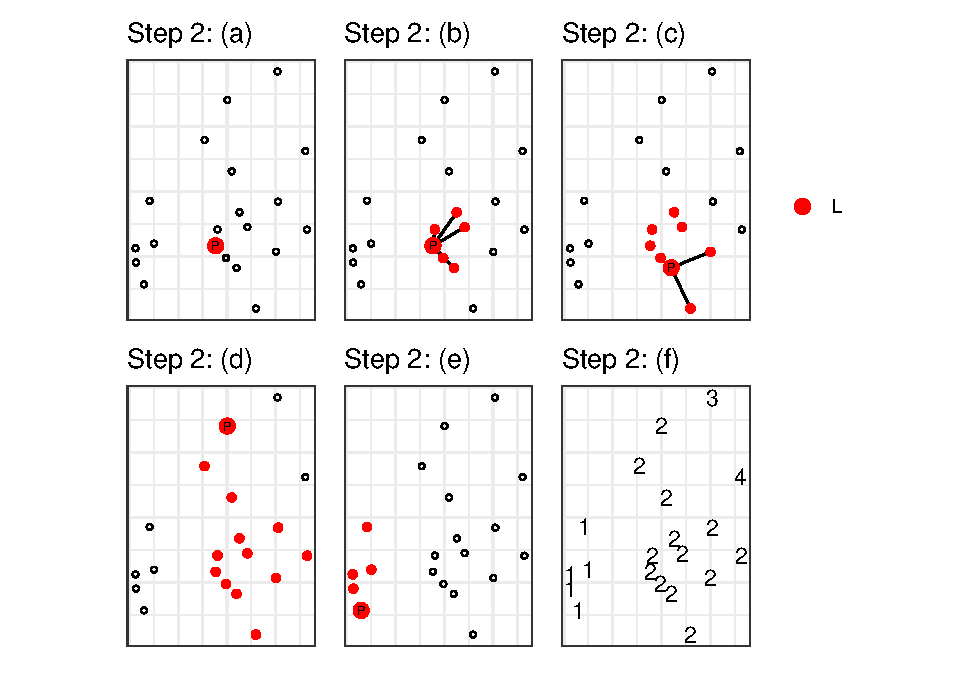
\includegraphics[width=0.8\linewidth]{clustering_paper_files/figure-latex/step2figs-1} 

}

\caption{An example of step 2 given 20 hotspots in interval $\boldsymbol{S}_t$. (a) A hotspot is selected randomly as the first item of list $\boldsymbol{L}$ and the pointer $\boldsymbol{P}$. Hotspots in list $\boldsymbol{L}$ are in red. Pointer $\boldsymbol{P}$ is drawn with larger marker size. (b) Nearby hotspots of the pointer $\boldsymbol{P}$ are appended to the list $\boldsymbol{L}$. (c) Move pointer $\boldsymbol{P}$ to the next item of list $\boldsymbol{L}$ and append the nearby hotspots to list $\boldsymbol{L}$. (d) The cluster is identified via repeating substep (c). (e) Clear the list $\boldsymbol{L}$, then randomly select an unassigned hotspot to identify another cluster. (f) The final clustering result is produced via repeating substep (d). The labels show the cluster each hotspot belongs to.}\label{fig:step2figs}
\end{figure}
\end{Schunk}

\textbf{3. Update memberships}

With spatial clustering results of each interval, the next step is to
update the memberships by bringing in information from earlier
intervals.

This step starts from \(t=2\) till \(t=T\). Given the interval
\(\boldsymbol{S}_t\), the algorithm will perform the following substeps:

\begin{enumerate}
\def\labelenumi{(\alph{enumi})}
\item
  Let \(h_i\) carries over from its membership in
  \(\boldsymbol{S}_{t-1}\), if \(h_i\) belongs to
  \(\boldsymbol{S}_{t-1}\), where \(h_i\) is the \(i\)th hotspot in the
  interval \(\boldsymbol{S}_t\). These hotspots are collected by a set
  \(\boldsymbol{H}_s = \{h_s^1,h_s^2,...\}\).
\item
  Let \(\boldsymbol{H}_c = \{h_c^1,h_c^2,...\}\), where \(h_c^i\) is the
  \(i\)th hotspot in set \(\boldsymbol{H}_c\) and \(h_c^i\) belongs to
  \(\boldsymbol{S}_t\) but does not belong to \(\boldsymbol{S}_{t-1}\).
  If \(h_c^i\) being clustered into the same component with \(h_s^j\) in
  interval \(\boldsymbol{S}_t\), let \(h_c^i\) carries over from the
  membership of the nearest \(h_s^j\), where \(h_s^j\) is the \(j\)th
  hotspot in the set \(\boldsymbol{H}_s\).
\end{enumerate}

Figure \ref{fig:step3figs} gives an example of this step.

\begin{Schunk}
\begin{figure}

{\centering 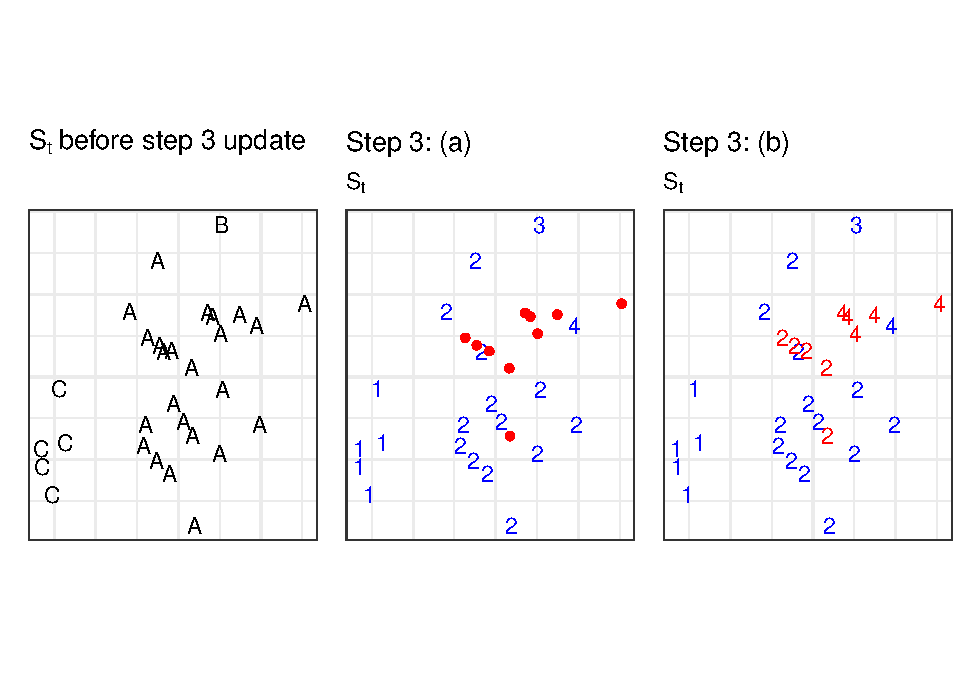
\includegraphics[width=0.8\linewidth]{clustering_paper_files/figure-latex/step3figs-1} 

}

\caption{An example of step 3. In this example, there are 30 hotspots belong to interval $\boldsymbol{S}_t$. (a) 20 out of 30 hotspots belong to both interval $\boldsymbol{S}_t$ and interval $\boldsymbol{S}_{t-1}$. Let these hotspots carry over from their memberships in $\boldsymbol{S}_{t-1}$. They are annotated in blue with membership labels. Points in red are the rest 10 hotspots that only belong to interval $\boldsymbol{S}_t$. (b) For each red point, let it carry over from the membership of the nearest blue label which shares the same component (according to the spatial clustering result of this interval) in interval $\boldsymbol{S}_t$. }\label{fig:step3figs}
\end{figure}
\end{Schunk}

\textbf{4. Handle noise}

After performing step 3, all membership labels will be produced.
However, a noticeable amount of small clusters could exist. We provide a
noise filter in the last step to address this issue.

Parameter \(minPts\) is the minimum number of hotspots a cluster
contains and parameter \(minTime\) is the minimum time a cluster lasts.
Any cluster that doesn't satisfy this two conditions will be assigned
with membership \(-1\) to indicate noise.

\hypertarget{result}{%
\subsubsection{Result}\label{result}}

The result of the spatiotemporal clustering algorithm applied on the
hotspot data is a vector of memberships with length equals to the number
of observations in the data.

\hypertarget{package}{%
\subsection{Package}\label{package}}

The implementation of our spatiotemporal algorithm is provided in the R
package \CRANpkg{spotoroo}. The released version can be installed from
CRAN.

\begin{verbatim}
install.packages("spotoroo")
\end{verbatim}

The following demonstration will assume the package \CRANpkg{spotoroo}
has been loaded.

\begin{verbatim}
library(spotoroo)
\end{verbatim}

\hypertarget{clustering-analysis}{%
\subsubsection{Clustering Analysis}\label{clustering-analysis}}

The main function of this package is \texttt{hotspot\_cluster()}, which
can be used to perform the spatiotemporal clustering algorithm on the
satellite hotspot data.

In this function, three different kinds of arguments need to be
specified. Arguments \texttt{hotspots}, \texttt{lon}, \texttt{lat}, and
\texttt{obsTime} are used to specify the hotspot data set and its
relevant columns. Arguments \texttt{activeTime}, \texttt{adjDist},
\texttt{minPts}, and \texttt{minTime} have already been defined in the
\protect\hyperlink{algorithm}{Algorithm} section. Besides, arguments
\texttt{timeUnit} and \texttt{timestep} are used to convert observed
time to discrete time index.

The following code is an example of the use of
\texttt{hotspot\_cluster()}. It set the \texttt{activeTime} to be \(24\)
time indexes, the \texttt{adjDist} to be \(3000\) meters, the
\texttt{minPts} to be \(4\) hotspots, the \texttt{minTime} to be \(3\)
time indexes, and \(1\) time index to be \(1\) hour.

\begin{Schunk}
\begin{Sinput}
result <- hotspot_cluster(hotspots = hotspots,
                          lon = "lon",
                          lat = "lat",
                          obsTime = "obsTime",
                          activeTime = 24,
                          adjDist = 3000,
                          minPts = 4,
                          minTime = 3,
                          timeUnit = "h",
                          timeStep = 1)
\end{Sinput}
\end{Schunk}

The output of this function is a \texttt{spotoroo} object, which is
actually a \texttt{list} contains a \texttt{data.frame} called
\texttt{hotspots}, a \texttt{data.frame} called \texttt{ignition}, and a
\texttt{list} called \texttt{setting}.

\begin{Schunk}
\begin{Sinput}
result
\end{Sinput}
\begin{Soutput}
#> i spotoroo object: 6 clusters | 1070 hot spots (including noise points)
\end{Soutput}
\end{Schunk}

The \texttt{hotspots} data set contains information of each hotspot.
Particularly, the \texttt{membership} column is the memberships.

\begin{Schunk}
\begin{Sinput}
head(result$hotspots, 2)
\end{Sinput}
\begin{Soutput}
#>      lon       lat             obsTime timeID membership noise distToIgnition
#> 1 147.46 -37.46000 2020-02-01 05:20:00    809         -1  TRUE              0
#> 2 146.48 -37.93999 2020-01-02 06:30:00     90         -1  TRUE              0
#>   distToIgnitionUnit timeFromIgnition timeFromIgnitionUnit
#> 1                  m   718.8333 hours                    h
#> 2                  m   718.8333 hours                    h
\end{Soutput}
\end{Schunk}

The \texttt{ignition} data set contains information of each cluster. The
\texttt{lon} and \texttt{lat} are the coordinate information of the
ignition points, which are the centroids of the earliest observed
hotspots of each cluster.

\begin{Schunk}
\begin{Sinput}
head(result$ignition, 2)
\end{Sinput}
\begin{Soutput}
#>   membership    lon    lat             obsTime timeID obsInCluster
#> 1          1 149.30 -37.77 2019-12-29 13:10:00      1          146
#> 2          2 146.72 -36.84 2020-01-08 01:40:00    229          165
#>   clusterTimeLen clusterTimeLenUnit
#> 1 116.1667 hours                  h
#> 2 148.3333 hours                  h
\end{Soutput}
\end{Schunk}

The generic function \texttt{summary()} can be used to get a brief
report of the clustering result.

\begin{verbatim}
summary(result)
\end{verbatim}

\hypertarget{extract-a-subset-of-clusters}{%
\subsubsection{Extract a subset of
clusters}\label{extract-a-subset-of-clusters}}

The function \texttt{extract\_fire()} enable user to convert a
\texttt{spotoroo} object to a \texttt{data.frame} for further analysis.
To keep all information from the clustering result including noise
points, set \texttt{noise\ =\ TRUE}.

\begin{Schunk}
\begin{Sinput}
all_fires <- extract_fire(result, noise = TRUE)
\end{Sinput}
\end{Schunk}

By providing a vector to the argument \texttt{cluster}, the function
will extract the corresponding clusters from the clustering result.

\begin{Schunk}
\begin{Sinput}
fire_1_and_2 <- extract_fire(result, cluster = c(1, 2), noise = FALSE)
\end{Sinput}
\end{Schunk}

\hypertarget{visualize-the-clustering-result}{%
\subsubsection{Visualize the clustering
result}\label{visualize-the-clustering-result}}

The \CRANpkg{spotoroo} provides three methods to visualize the
clustering result. They all can be produced by the generic function
\texttt{plot()}.

The default plot produced by the function is a scatter plot of the
clsuters and their ignition locations showing the spatial distribution
of the fires.

\begin{Schunk}
\begin{Sinput}
plot(result)
\end{Sinput}


\begin{center}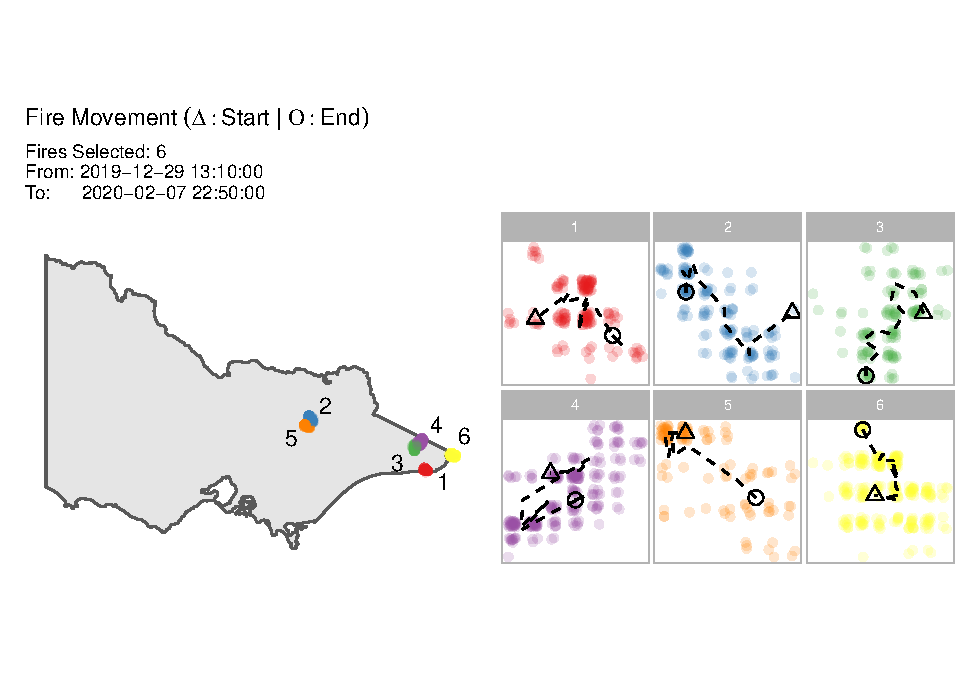
\includegraphics[width=0.8\linewidth]{clustering_paper_files/figure-latex/unnamed-chunk-10-1} \end{center}

\end{Schunk}

The path of the fire movement can be produced by setting
\texttt{type\ =\ \textquotesingle{}mov\textquotesingle{}}. The argument
\texttt{step} controls the time difference between successive step. The
movement can be also obtained from the \texttt{get\_fire\_mov()}
function.

\begin{Schunk}
\begin{Sinput}
plot(result, type = "mov", step = 6)
\end{Sinput}


\begin{center}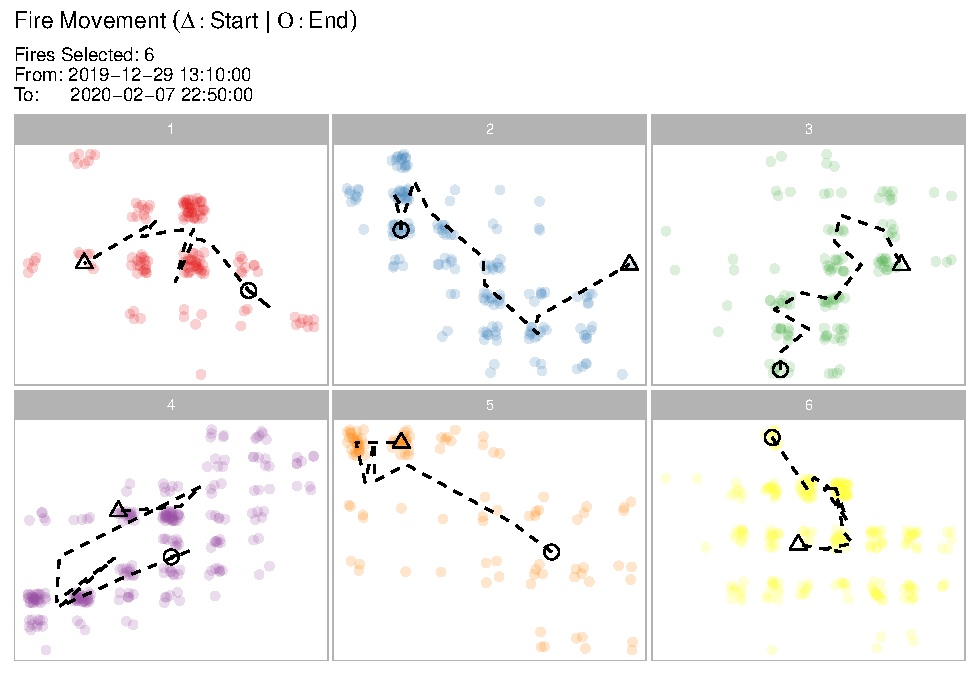
\includegraphics[width=0.8\linewidth]{clustering_paper_files/figure-latex/unnamed-chunk-11-1} \end{center}

\end{Schunk}

The time line of clusters can be produced by setting
\texttt{type\ =\ \textquotesingle{}timeline\textquotesingle{}} It could
be used to study the intensity of fire periods.

\begin{Schunk}
\begin{Sinput}
plot(result, type = "timeline")
\end{Sinput}


\begin{center}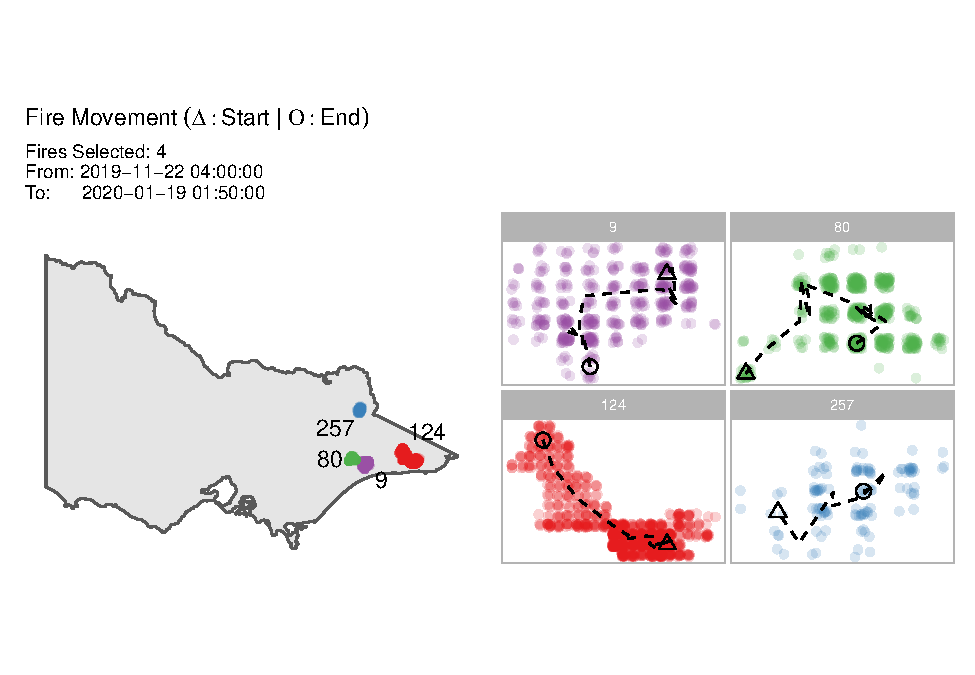
\includegraphics[width=0.8\linewidth]{clustering_paper_files/figure-latex/unnamed-chunk-12-1} \end{center}

\end{Schunk}

\hypertarget{application}{%
\subsection{Application}\label{application}}

In this section, an application will be illustrated to show how this
algorithm can be used to study bushfire ignition.

\hypertarget{data-source}{%
\subsubsection{Data source}\label{data-source}}

The following illustration will use the wild fire product (produced from
Himawari-8) supplied by the P-Tree System, Japan Aerospace Exploration
Agency (JAXA) \citeyearpar{jaxa} as the data source. This wild fire
product will be referred as the Himawari-8 hotspot data in the rest of
the paper. It contains records of 1989572 hotspots from October 2019 to
March 2020 in the full disk of 140 \textdegree east longitude with 0.02
\textdegree spatial resolution and 10 minutes temporal resolution.

The data pre-processing procedure includes selecting hotspots within the
boundary of Victoria and filtering hotspots with a threshold (irradiance
over 100 watts per square metre) suggested by landscape ecologist and
spatial scientist Dr.~Grant Williamson \citeyearpar{hotspots} to reduce
noise from the background.

The final hotspot data set contains 75936 observations with ID,
longitude, latitude and observed date as fields. The overall
distribution of these hotspots is shown in Figure \ref{fig:hotspots}.

\begin{Schunk}
\begin{figure}

{\centering 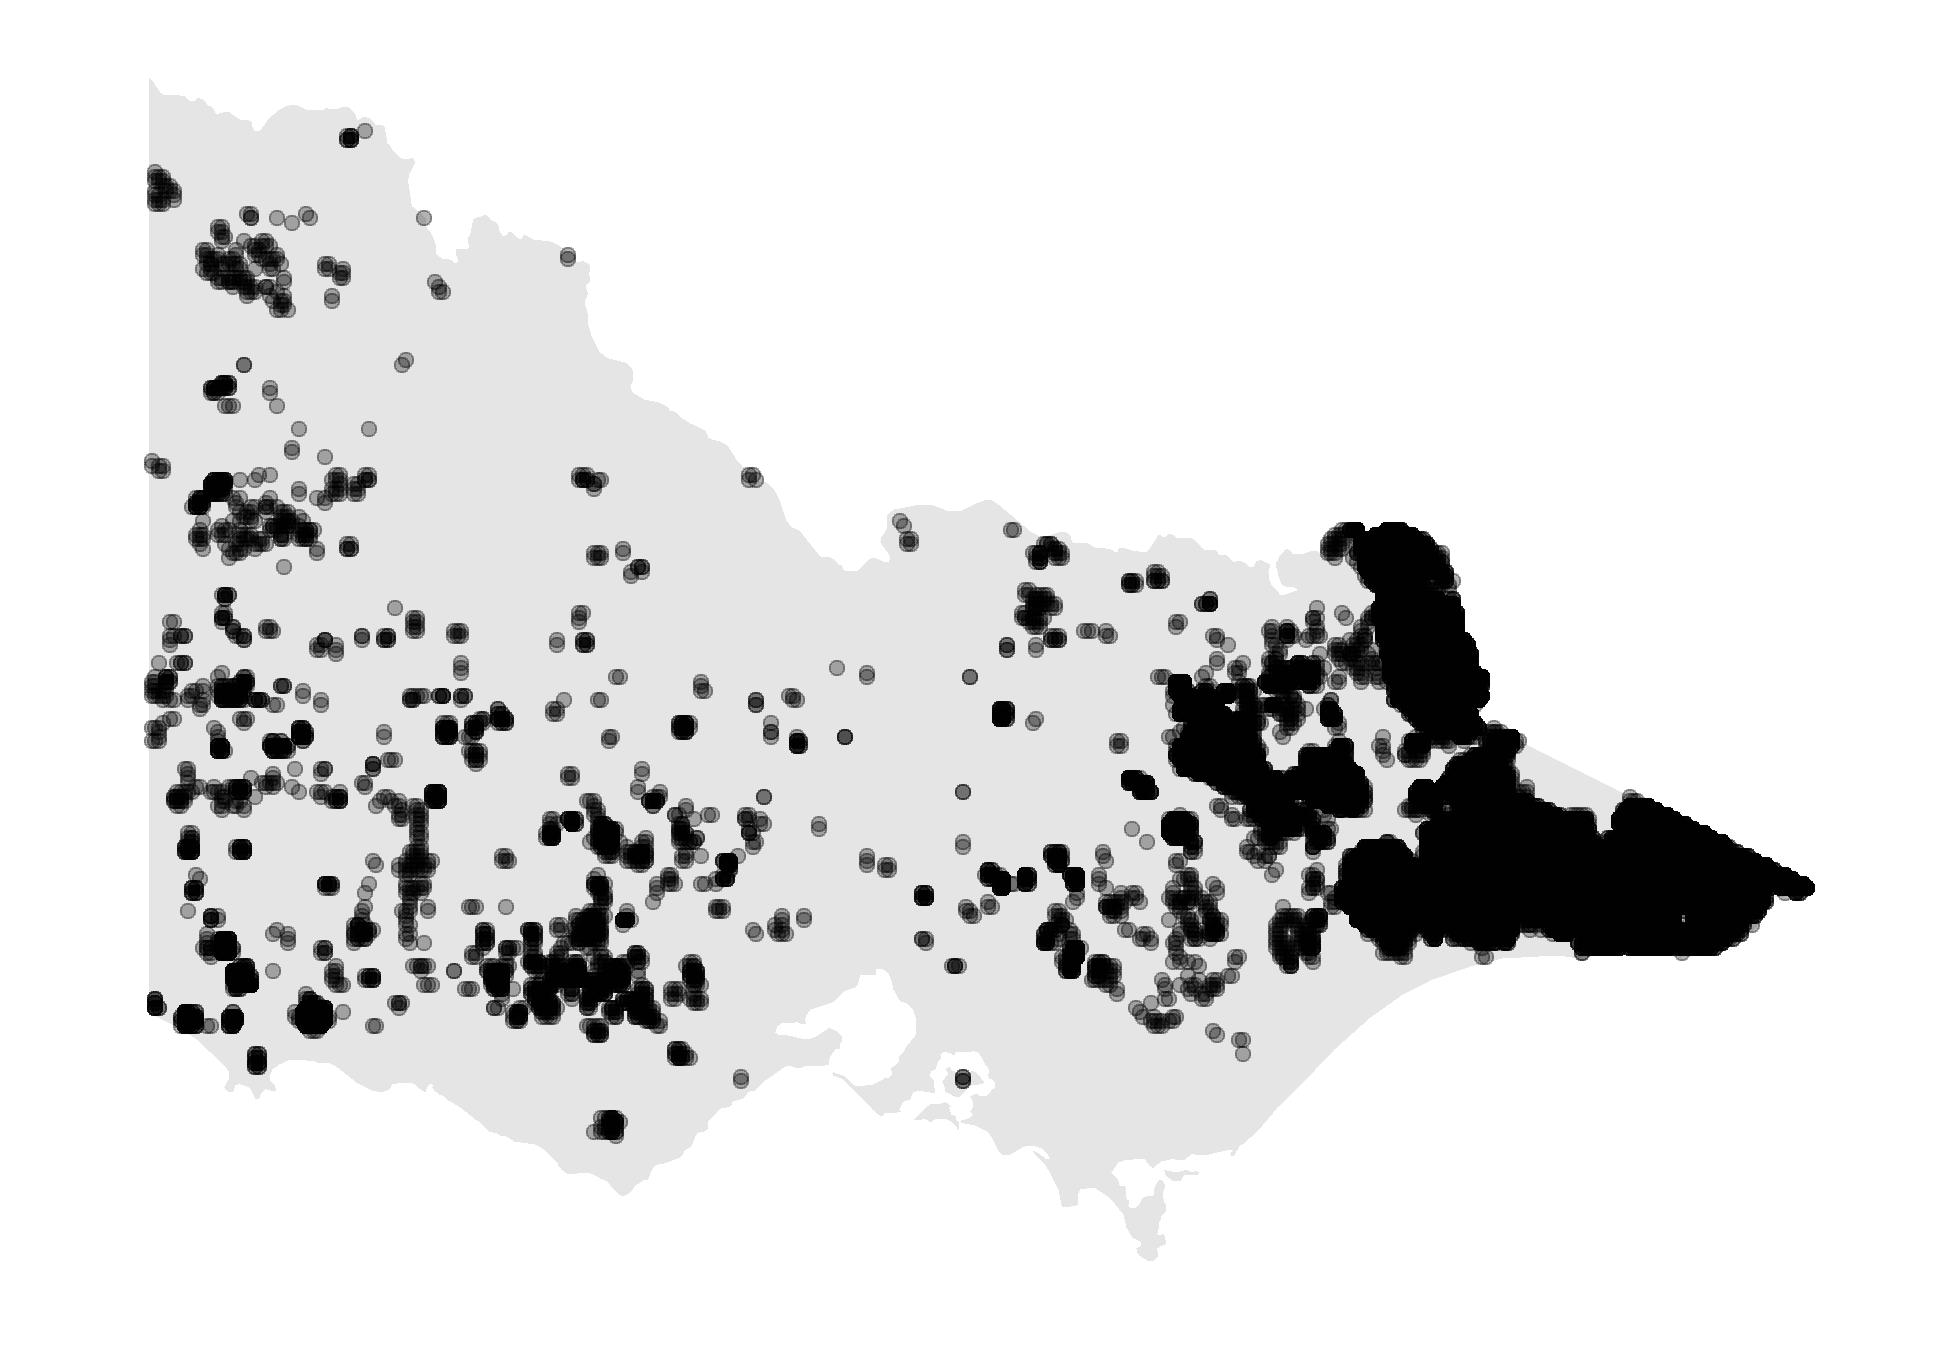
\includegraphics[width=0.8\linewidth]{figures/before_clustering} 

}

\caption[The distribution of hotspots in Victoria during 2019-2020 Australia bushfire season]{The distribution of hotspots in Victoria during 2019-2020 Australia bushfire season.}\label{fig:hotspots}
\end{figure}
\end{Schunk}

\hypertarget{clustering-the-himawari-8-hotspots}{%
\subsubsection{Clustering the Himawari-8
hotspots}\label{clustering-the-himawari-8-hotspots}}

To perform the clustering algorithm on the Himawari-8 hotspot data, we
first transform the observed time to time index by setting the time
difference between two successive index to be \(1\) hour. Then, set
\texttt{activeTime} to be \(24\) time indexes, \texttt{adjDist} to be
\(3000\) memters, \texttt{minPts} to be \(3\) hotspots and
\texttt{minTime} to be \(3\) indexes for the algorithm. The choice of
these parameters will be justified in the section ???.

\begin{verbatim}
result <- hotspot_cluster(hotspots = him_hotspots,
                            lon = "lon",
                            lat = "lat",
                            obsTime = "obsTime",
                            activeTime = 24,
                            adjDist = 3000,
                            minPts = 4,
                            minTime = 3,
                            timeUnit = "h",
                            timeStep = 1)
\end{verbatim}

The clustering result shows that 407 bushfires are found from 75936
hotspots.

\begin{Schunk}
\begin{Sinput}
result
\end{Sinput}
\begin{Soutput}
#> i spotoroo object: 407 clusters | 75936 hot spots (including noise points)
\end{Soutput}
\end{Schunk}

\hypertarget{determining-the-ignition-point-and-time-for-individual-fires}{%
\subsubsection{Determining the ignition point and time for individual
fires}\label{determining-the-ignition-point-and-time-for-individual-fires}}

Based on the clustering result, ignition location for each cluster can
be computed. The strategy is to select the earliest hotspot of a cluster
as its ignition point. Besides, if there are multiple earliest hotspots
belong to the same cluster, the centroids of these hotspots are used as
the ignition locations. According to this method, ignition points over 6
months can be produced using

\begin{verbatim}
plot(result, bg = plot_vic_map(), hotspot = FALSE)
\end{verbatim}

The result is given in Figure \ref{fig:clusteringfinalresults}.

And the ignited time of each fire can be produced using

\begin{verbatim}
plot(result, type = "timeline", mainBreak = "1 month", dateLabel = "%b %d, %y")`. 
\end{verbatim}

The result is given in Figure \ref{fig:himtimeline}.

\begin{Schunk}
\begin{figure}

{\centering 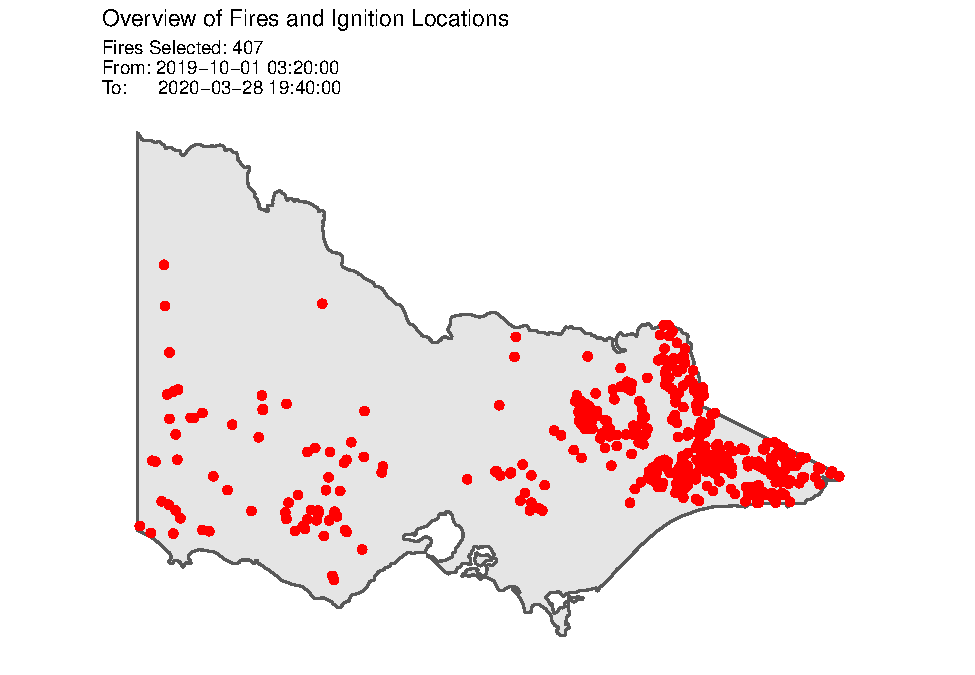
\includegraphics[width=0.8\linewidth]{clustering_paper_files/figure-latex/clusteringfinalresults-1} 

}

\caption[ The distribution of bushfire ignitions in Victoria during 2019-2020 Australian bushfire season]{ The distribution of bushfire ignitions in Victoria during 2019-2020 Australian bushfire season.}\label{fig:clusteringfinalresults}
\end{figure}
\end{Schunk}

\begin{Schunk}
\begin{figure}

{\centering 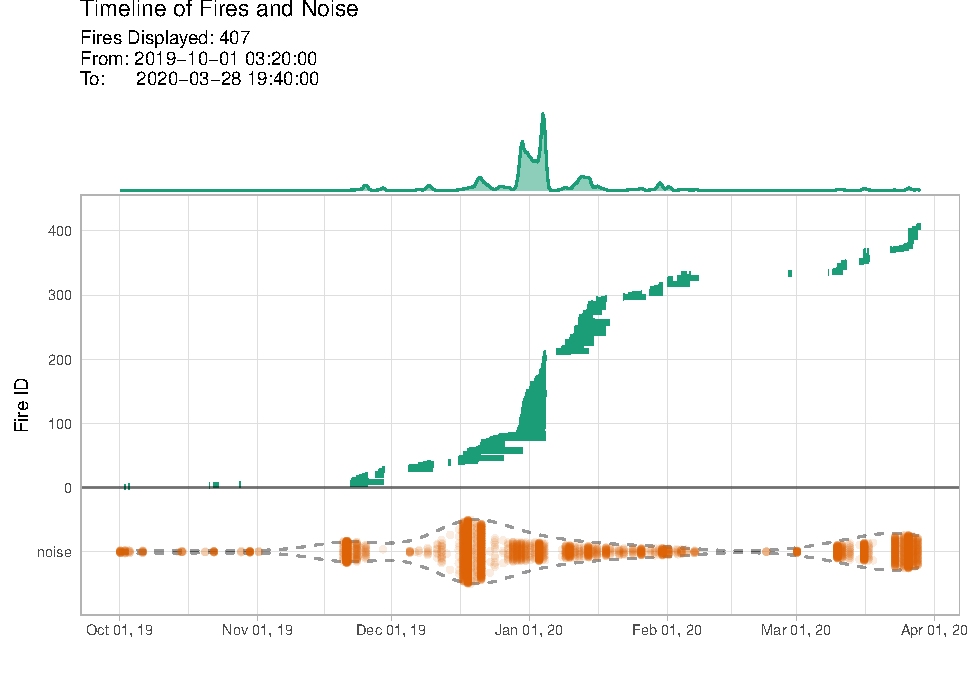
\includegraphics[width=0.8\linewidth]{clustering_paper_files/figure-latex/himtimeline-1} 

}

\caption[Timeline of 2019-2020 Victorian bushfire season]{Timeline of 2019-2020 Victorian bushfire season.}\label{fig:himtimeline}
\end{figure}
\end{Schunk}

\hypertarget{tracking-fire-movement}{%
\subsubsection{Tracking fire movement}\label{tracking-fire-movement}}

Display showing how a fire moves over time, maybe two or more fires

\begin{Schunk}


\begin{center}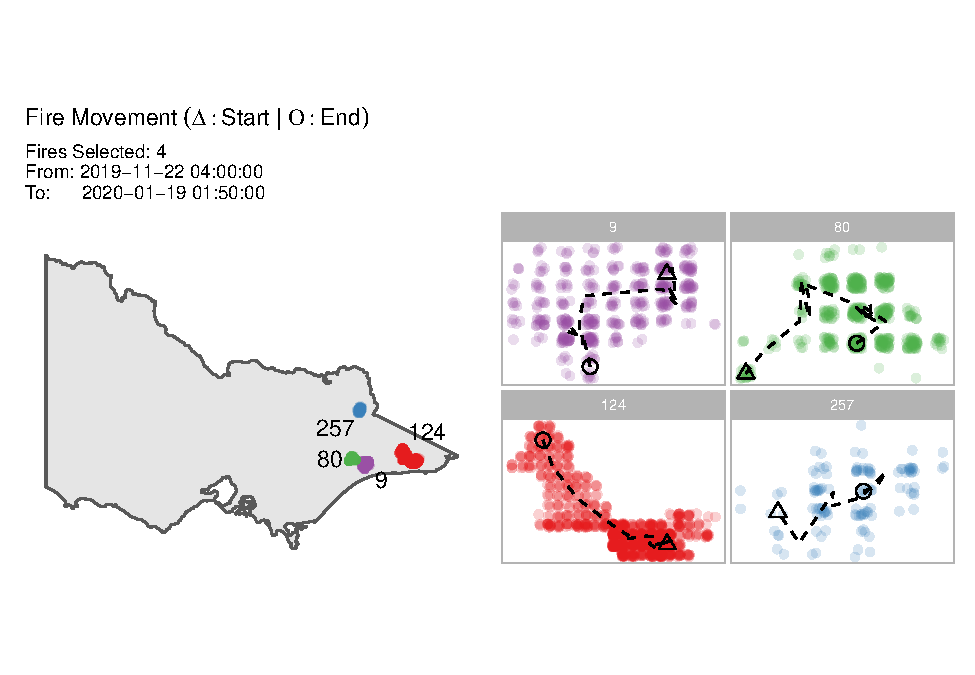
\includegraphics[width=0.8\linewidth]{clustering_paper_files/figure-latex/unnamed-chunk-15-1} \end{center}

\end{Schunk}

\hypertarget{allocating-resources-for-future-fire-prevention}{%
\subsubsection{Allocating resources for future fire
prevention}\label{allocating-resources-for-future-fire-prevention}}

Merging data with camp sites, CFA, roads, \ldots{}

\hypertarget{effects-of-parameter-choices}{%
\subsubsection{Effects of parameter
choices}\label{effects-of-parameter-choices}}

There are two parameters that being introduced in the outline of the
algorithm, which are \(AdjDist\) and \(ActiveTime\). The optimal choice
of these two parameters is not known but can be tuned using a
visualization tool.

Considering the relationships between \(AdjDist\), \(ActiveTime\) and
the number of clusters in the clustering result, increase either
\(AdjDist\) or \(ActiveTime\) will usually reduce the number of
clusters. However, if there are large gaps between clusters spatially
and temporally, increase these two parameters will not significantly
reduce the number of clusters. Given one of the metrics to evaluate the
goodness of the clustering result is the gap between clusters, the
optimal choice of \(AdjDist\) and \(ActiveTime\) can be chosen when they
have minimum impact on the number of clusters. However, under this
setting, the optimal \(ActiveTime\) and \(AdjDist\) will approach to
infinitely as the number of clusters approach to 1. Hence, a restriction
needs to be applied on this optimization. Increase of \(ActiveTime\) and
\(AdjDist\) will only be allowed when there is a major fall of the
number of clusters. Based on this rule, a visualization tool inspired by
the scree plot used in the principal component analysis is developed.
Similar to the scree plot, users need to determine the \(ActiveTime\)
and \(AdjDist\) to capture most of the decrease of the number of
clusters. Figure \ref{fig:vis1} and \ref{fig:vis2} show the parameter
tuning process by using this visualization tool. The final choice of
\(ActiveTime\) is \(24\) hours and \(AdjDist\) is \(3000\) metres.

\begin{Schunk}
\begin{figure}

{\centering 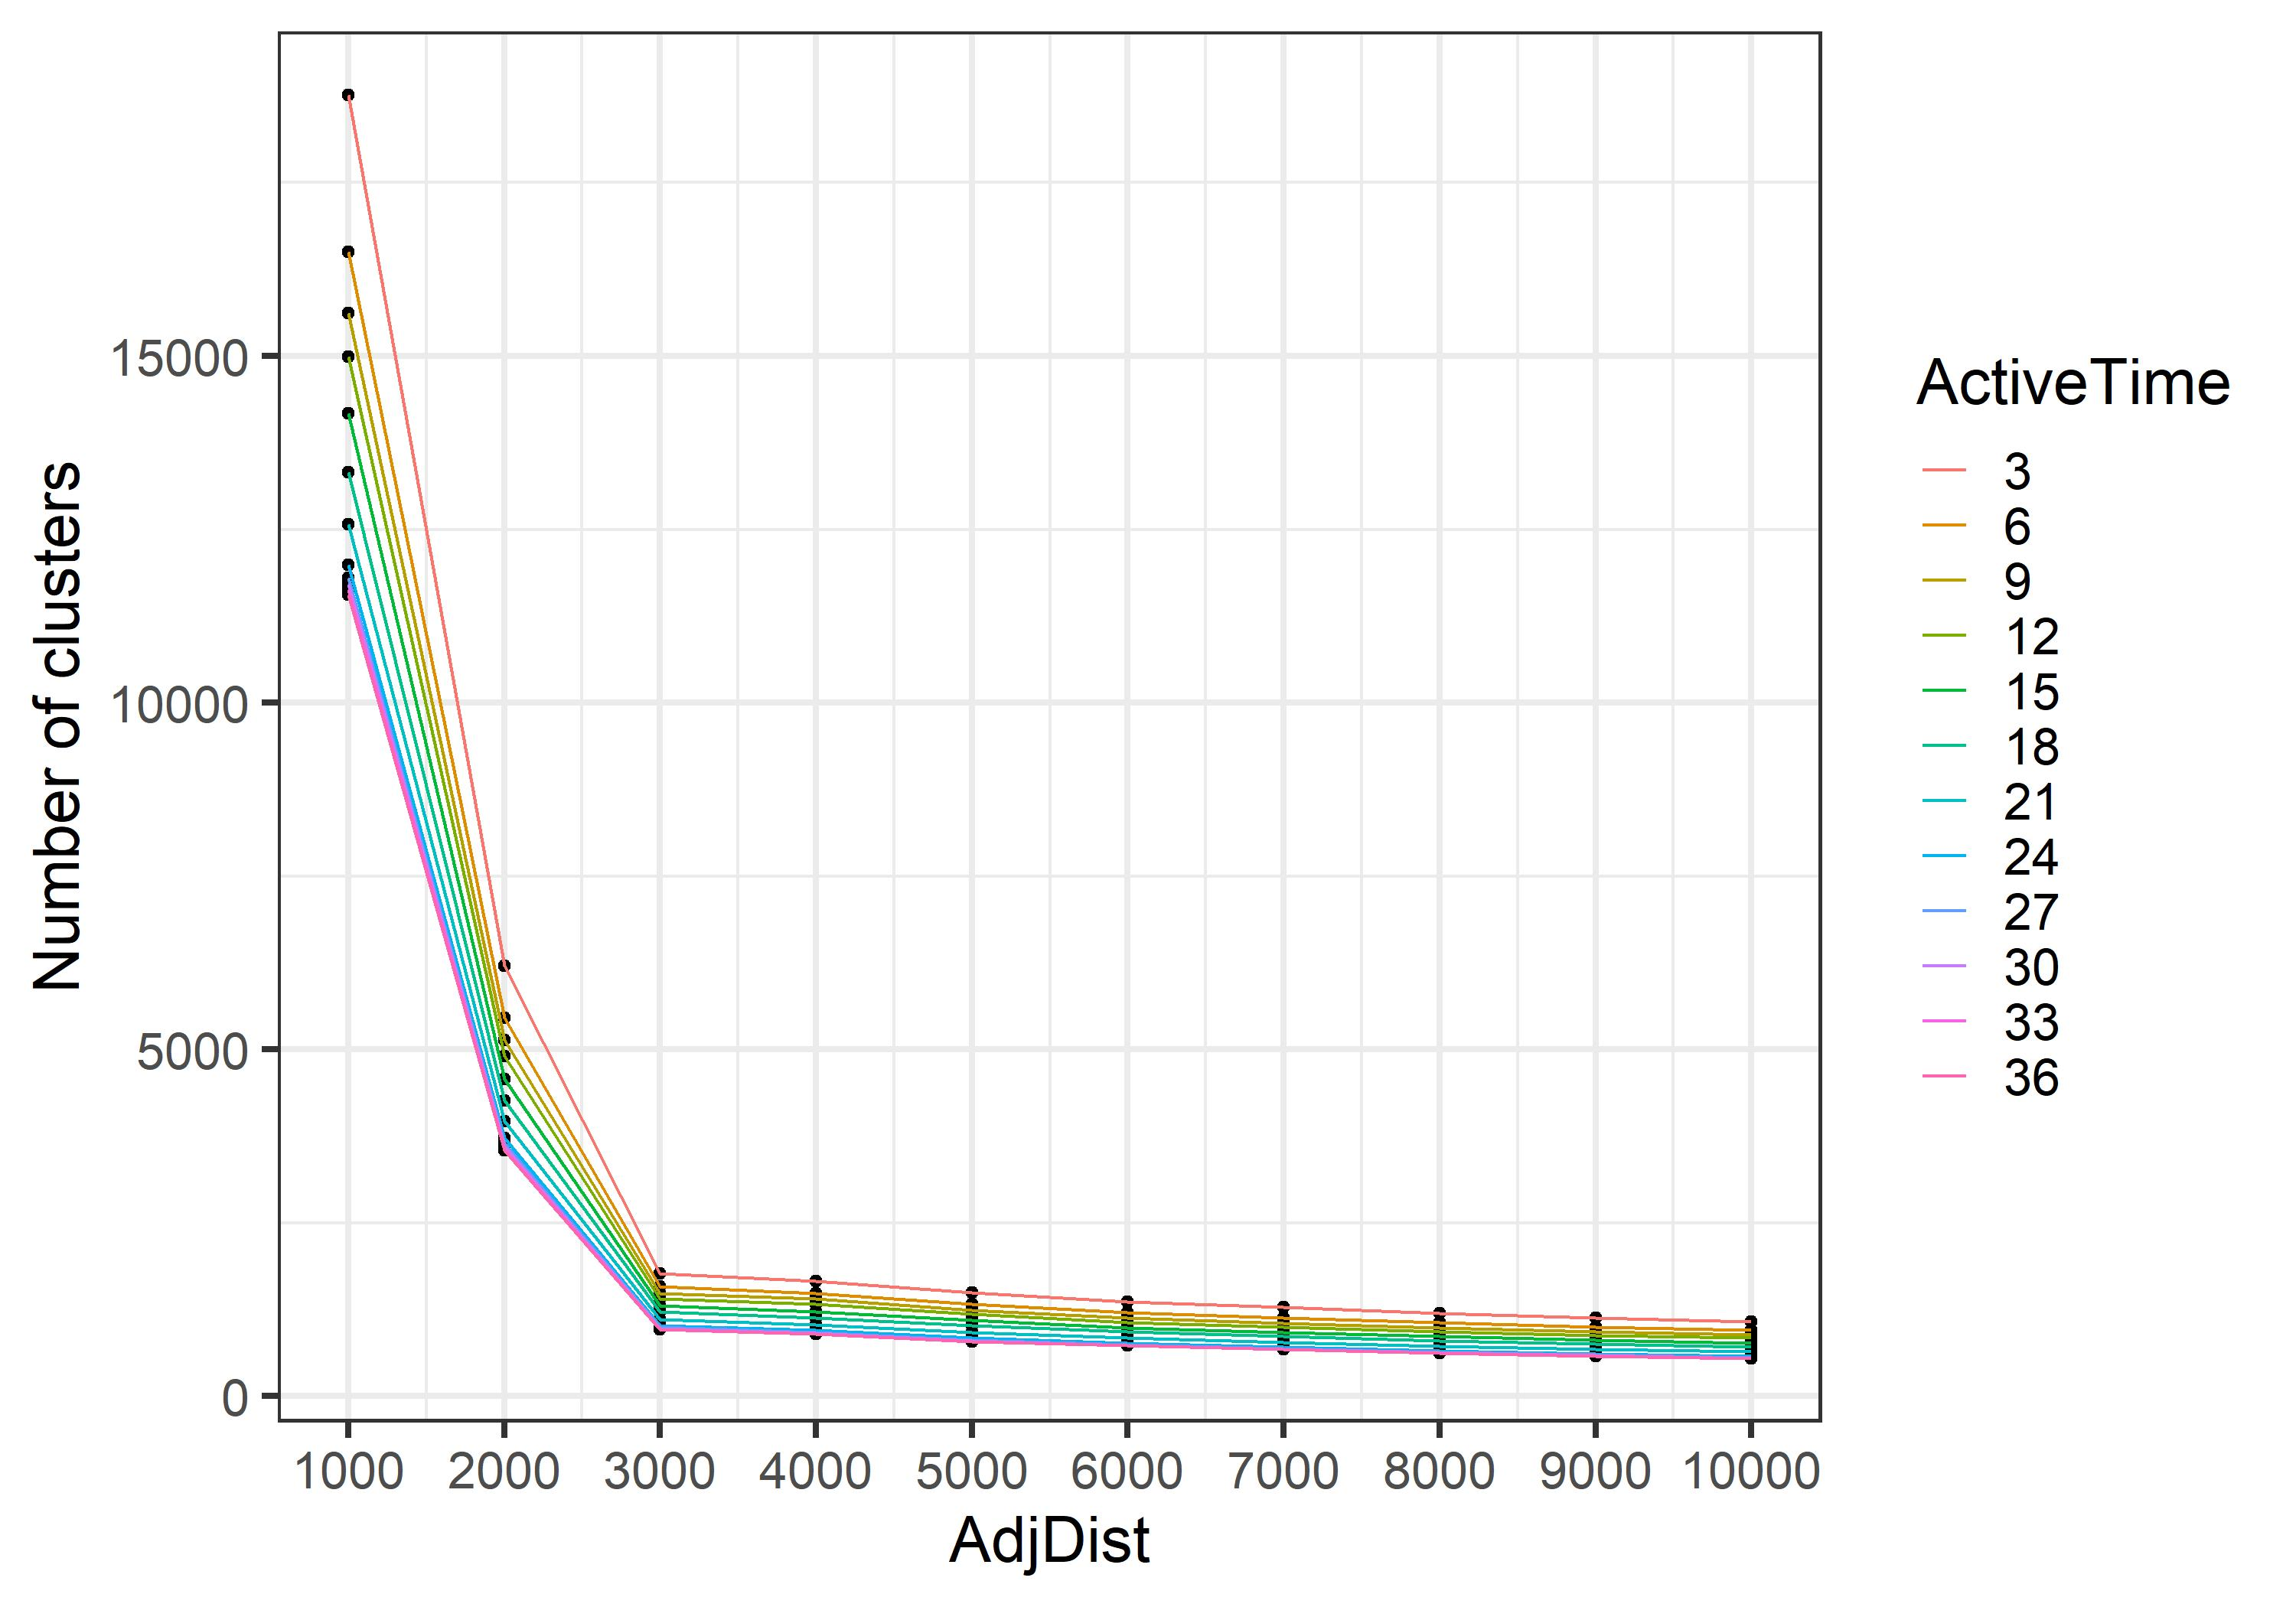
\includegraphics[width=0.8\linewidth]{figures/clustering_tuning_1} 

}

\caption[A visualization tool for parameter tuning ]{A visualization tool for parameter tuning . It works like a scree plot. Major falls of the number of clusters are observed when $AdjDist < 3000$ so the reasonable choice of $AdjDist$ is 3000m.}\label{fig:vis1}
\end{figure}
\end{Schunk}

\begin{Schunk}
\begin{figure}

{\centering 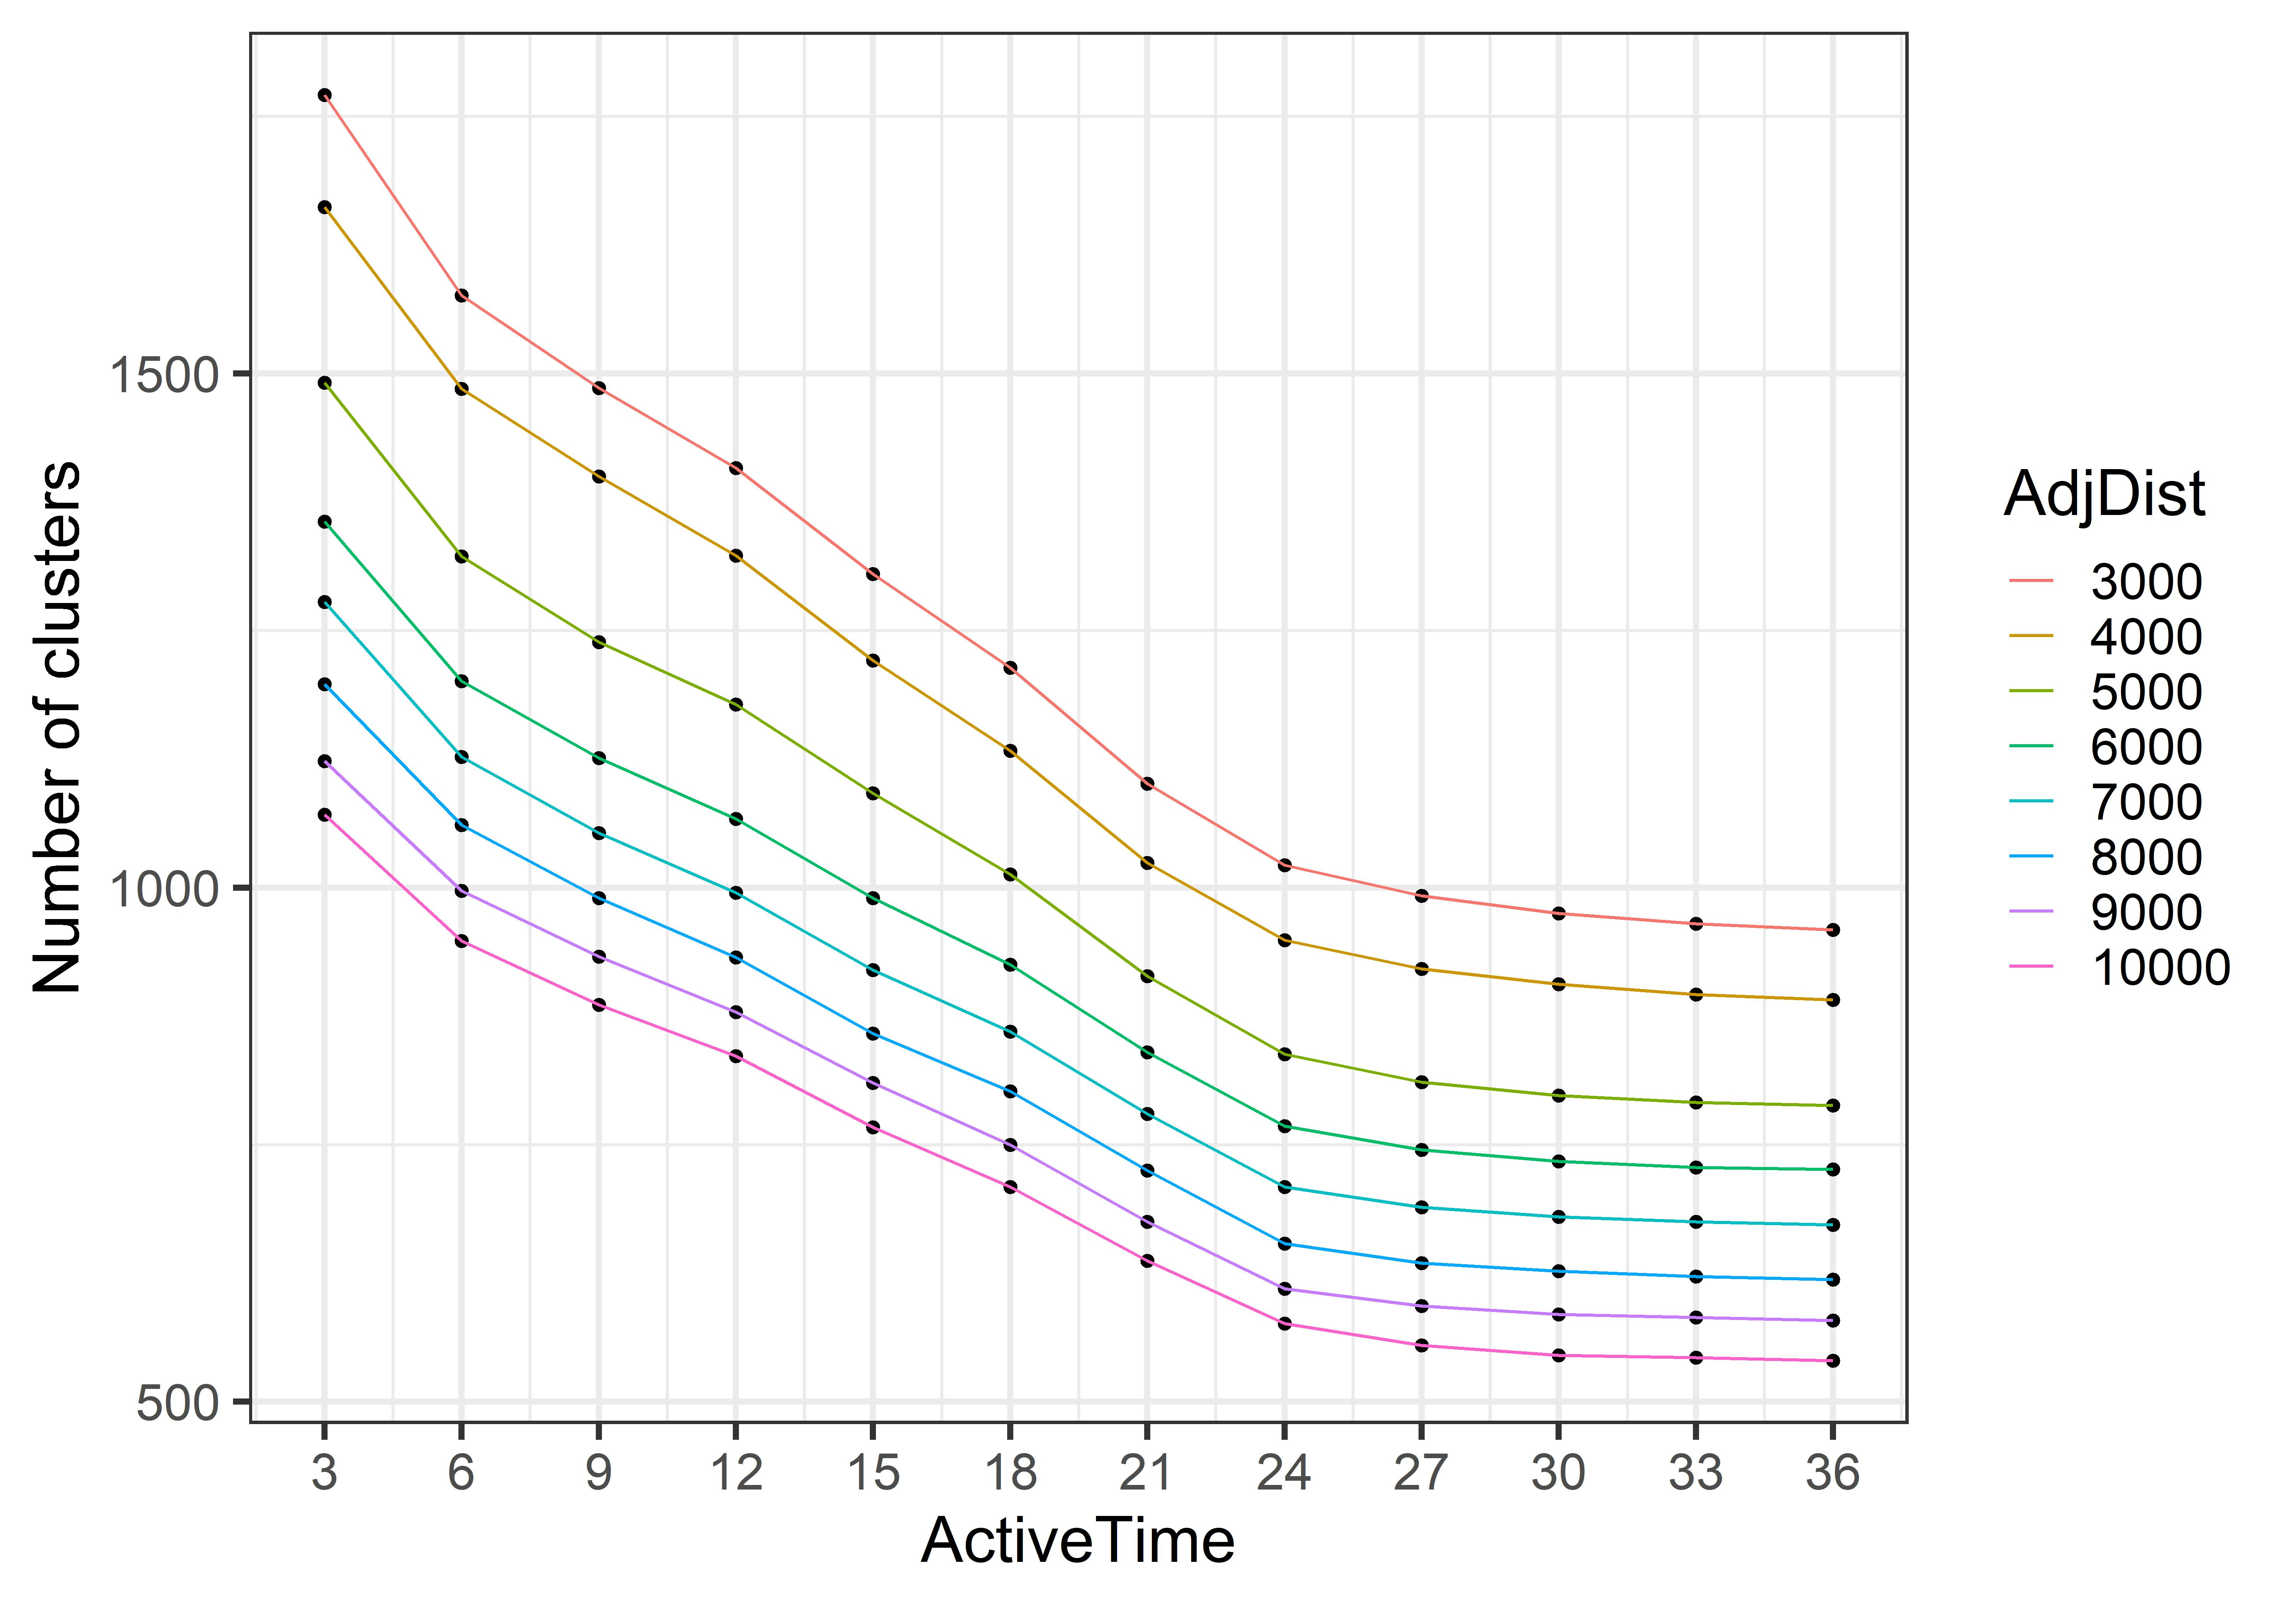
\includegraphics[width=0.8\linewidth]{figures/clustering_tuning_2} 

}

\caption[Major falls of the number of clusteres are observed when $ActiveTime < 24$, so the reasonable choice of $ActiveTime$ is 24 hours]{Major falls of the number of clusteres are observed when $ActiveTime < 24$, so the reasonable choice of $ActiveTime$ is 24 hours.}\label{fig:vis2}
\end{figure}
\end{Schunk}

\hypertarget{summary}{%
\subsection{Summary}\label{summary}}

\bibliography{RJreferences}


\address{%
Weihao Li\\
Monash University\\%
Econometrics and Business Statistics\\
%
%
%
\\\href{mailto:weihao.li@monash.edu}{\nolinkurl{weihao.li@monash.edu}}
}

\address{%
Emily Dodwell\\
??\\%
line 1\\ line 2\\
%
%
%
\\\href{mailto:emdodwell@gmail.com}{\nolinkurl{emdodwell@gmail.com}}
}

\address{%
Dianne Cook\\
Monash University\\%
Econometrics and Business Statistics\\
%
%
%
\\\href{mailto:dicook@monash.edu}{\nolinkurl{dicook@monash.edu}}
}
